\documentclass[DIN, pagenumber=false, fontsize=11pt, parskip=half]{scrartcl}

\usepackage{amsmath}
\usepackage{amsfonts}
\usepackage{amssymb}
\usepackage{enumitem}
\usepackage[utf8]{inputenc} 
\usepackage[ngerman]{babel} 
\usepackage[T1]{fontenc} 
\usepackage{pgfplots}
\usepackage{xcolor}
\usepackage{listings}
\usepackage{float}
\usepackage{graphicx}
\usepackage{booktabs}
\usepackage{tkz-euclide}
\usepackage{svg}

\definecolor{mygreen}{RGB}{28,172,0} % color values Red, Green, Blue
\definecolor{mylilas}{RGB}{170,55,241}

\DeclareUnicodeCharacter{3B4}{\ensuremath{\delta}}

\tikzstyle{neuron}=[circle,fill=black!25,minimum size=30pt,inner sep=0pt]

\lstset{language=Matlab,%
    %basicstyle=\color{red},
    breaklines=true,%
    morekeywords={matlab2tikz},
    keywordstyle=\color{blue},%
    morekeywords=[2]{1}, keywordstyle=[2]{\color{black}},
    identifierstyle=\color{black},%
    stringstyle=\color{mylilas},
    commentstyle=\color{mygreen},%
    showstringspaces=false,%without this there will be a symbol in the places where there is a space
    numbers=left,%
    numberstyle={\tiny \color{black}},% size of the numbers
    numbersep=9pt, % this defines how far the numbers are from the text
    emph=[1]{for,end,break},emphstyle=[1]\color{red}, %some words to emphasise
    %emph=[2]{word1,word2}, emphstyle=[2]{style},    
}

\title{Einführung in die Neuroinformatik}
\author{Tim Luchterhand, Paul Nykiel (Gruppe P)}

\begin{document}
    \maketitle
    \section{Backpropagation [Pen and Paper]}
    \begin{enumerate}
        \item Forwärts propagieren:
            \begin{eqnarray*}
                u_1^{(1)} &=& x_1 \cdot w_{11}^{(1)} + x_2 \cdot w_{21}^{(1)} + b_1^{(1)}\\
                y_1^{(1)} &=& f_1(u_1^{(1)}) \\
                u_1^{(2)} &=& y_1^{(1)} \cdot w_{11}^{(2)} + y_2^{(1)} \cdot w_{21}^{(2)} + b_1^{(2)}\\
                y_1^{(2)} &=& f_2(u_1^{(2)}) 
            \end{eqnarray*}
        \item Fehler in der Ausgabeschicht bestimmen:
            \begin{eqnarray*}
                \delta_1^{(2)} &=& y_1^{(2)} - T_1
            \end{eqnarray*}
        \item Backpropagation
            \begin{eqnarray*}
                \delta_1^{(1)} &=& \delta_1^{(2)} w_{11}^{(2)}f'\left(u_i^{(1)}\right)
            \end{eqnarray*}
        \item Gewichte adaptieren
            \begin{equation*}
                \tilde{w_{11}^{(1)}} =  w_{11}^{(1)} + \eta x_1 \delta_1^{(1)}
            \end{equation*}
    \end{enumerate}
    
	\begin{figure}[H]
		\centering
		\includesvg[width=\textwidth]{Blatt5A1}
		\caption{Ablauf graphisch dargestellt}
	\end{figure} 

    \section{Backpropagation [Matlab]}
    \subsection{}
    \lstinputlisting{initWeights.m}
    \subsection{}
    \lstinputlisting{forward.m}
    \subsection{}
    \lstinputlisting{propagateError.m}
    \lstinputlisting{transDiff.m}
    \subsection{}
    \lstinputlisting{train.m}
    \subsection{}
    \lstinputlisting{b05a02.m}
    \begin{figure}[H]
        \centering
        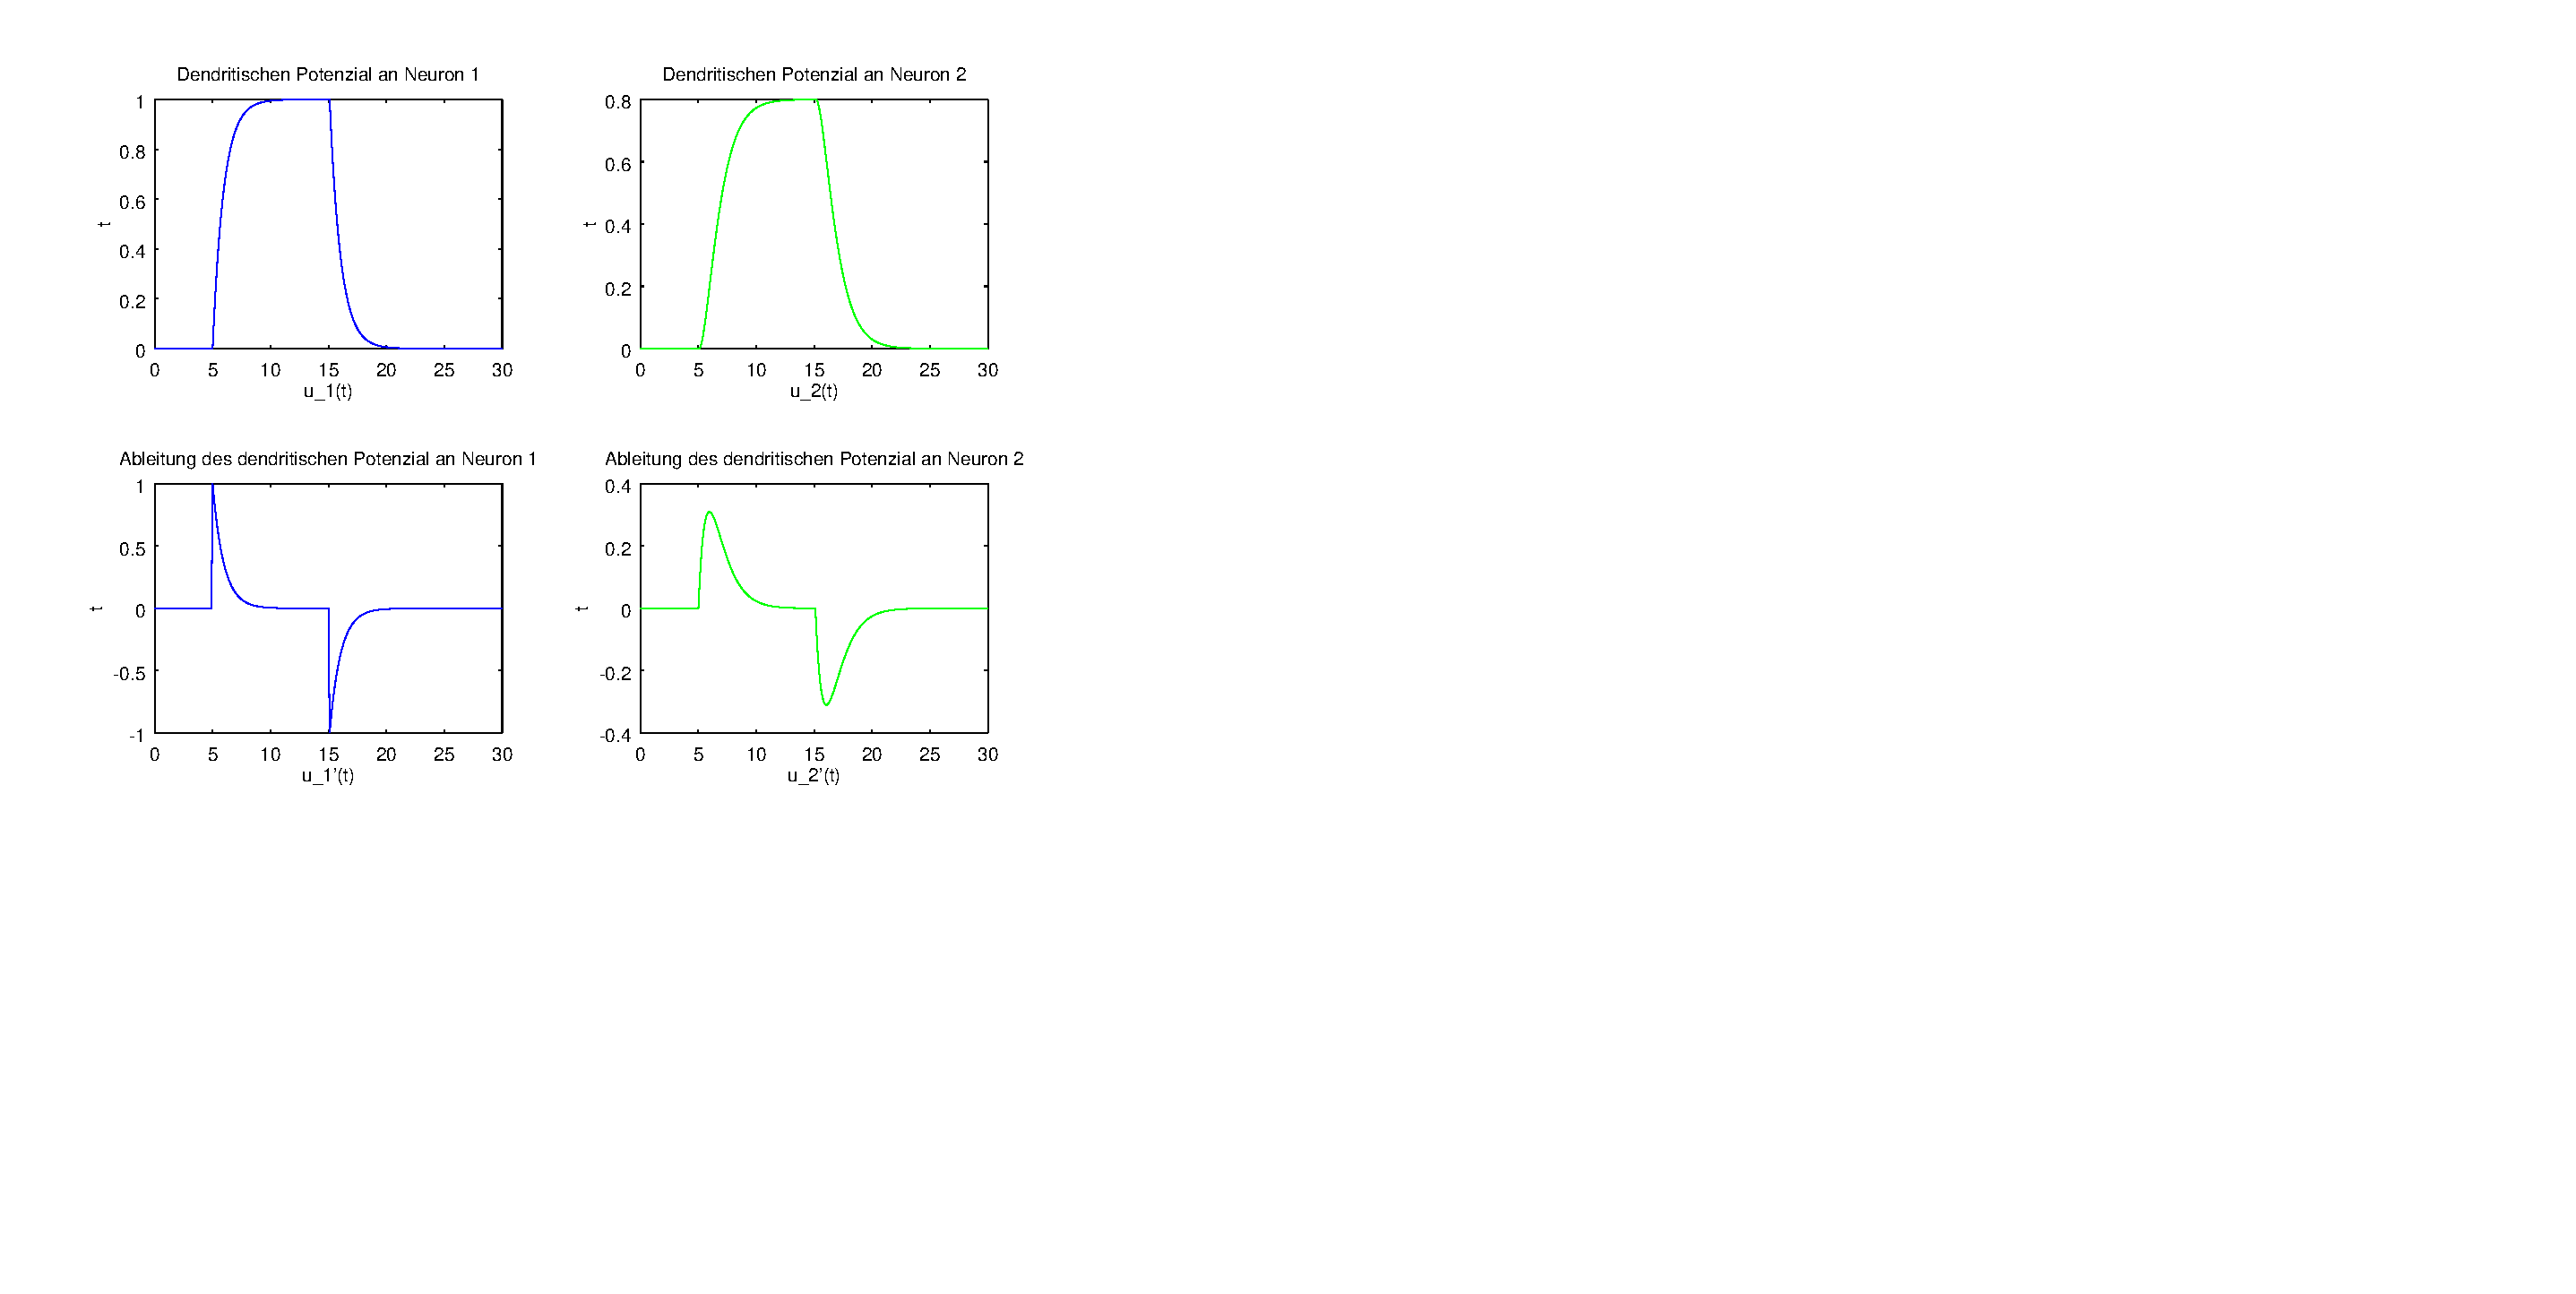
\includegraphics[trim = {0 9cm 27cm 0}, clip,width=\textwidth]{Plot}
        \caption{Ausgabe des Matlab-Skripts} 
    \end{figure}
\end{document}
